\documentclass[ignorenonframetext,]{beamer}
\setbeamertemplate{caption}[numbered]
\setbeamertemplate{caption label separator}{: }
\setbeamercolor{caption name}{fg=normal text.fg}
\beamertemplatenavigationsymbolsempty
\usepackage{lmodern}
\usepackage{amssymb,amsmath}
\usepackage{ifxetex,ifluatex}
\usepackage{fixltx2e} % provides \textsubscript
\ifnum 0\ifxetex 1\fi\ifluatex 1\fi=0 % if pdftex
  \usepackage[T1]{fontenc}
  \usepackage[utf8]{inputenc}
\else % if luatex or xelatex
  \ifxetex
    \usepackage{mathspec}
  \else
    \usepackage{fontspec}
  \fi
  \defaultfontfeatures{Ligatures=TeX,Scale=MatchLowercase}
\fi
% use upquote if available, for straight quotes in verbatim environments
\IfFileExists{upquote.sty}{\usepackage{upquote}}{}
% use microtype if available
\IfFileExists{microtype.sty}{%
\usepackage{microtype}
\UseMicrotypeSet[protrusion]{basicmath} % disable protrusion for tt fonts
}{}
\newif\ifbibliography
\hypersetup{
            pdfborder={0 0 0},
            breaklinks=true}
\usepackage{color}
\usepackage{fancyvrb}
\newcommand{\VerbBar}{|}
\newcommand{\VERB}{\Verb[commandchars=\\\{\}]}
\DefineVerbatimEnvironment{Highlighting}{Verbatim}{commandchars=\\\{\}}
% Add ',fontsize=\small' for more characters per line
\usepackage{framed}
\definecolor{shadecolor}{RGB}{248,248,248}
\newenvironment{Shaded}{\begin{snugshade}}{\end{snugshade}}
\newcommand{\KeywordTok}[1]{\textcolor[rgb]{0.13,0.29,0.53}{\textbf{{#1}}}}
\newcommand{\DataTypeTok}[1]{\textcolor[rgb]{0.13,0.29,0.53}{{#1}}}
\newcommand{\DecValTok}[1]{\textcolor[rgb]{0.00,0.00,0.81}{{#1}}}
\newcommand{\BaseNTok}[1]{\textcolor[rgb]{0.00,0.00,0.81}{{#1}}}
\newcommand{\FloatTok}[1]{\textcolor[rgb]{0.00,0.00,0.81}{{#1}}}
\newcommand{\ConstantTok}[1]{\textcolor[rgb]{0.00,0.00,0.00}{{#1}}}
\newcommand{\CharTok}[1]{\textcolor[rgb]{0.31,0.60,0.02}{{#1}}}
\newcommand{\SpecialCharTok}[1]{\textcolor[rgb]{0.00,0.00,0.00}{{#1}}}
\newcommand{\StringTok}[1]{\textcolor[rgb]{0.31,0.60,0.02}{{#1}}}
\newcommand{\VerbatimStringTok}[1]{\textcolor[rgb]{0.31,0.60,0.02}{{#1}}}
\newcommand{\SpecialStringTok}[1]{\textcolor[rgb]{0.31,0.60,0.02}{{#1}}}
\newcommand{\ImportTok}[1]{{#1}}
\newcommand{\CommentTok}[1]{\textcolor[rgb]{0.56,0.35,0.01}{\textit{{#1}}}}
\newcommand{\DocumentationTok}[1]{\textcolor[rgb]{0.56,0.35,0.01}{\textbf{\textit{{#1}}}}}
\newcommand{\AnnotationTok}[1]{\textcolor[rgb]{0.56,0.35,0.01}{\textbf{\textit{{#1}}}}}
\newcommand{\CommentVarTok}[1]{\textcolor[rgb]{0.56,0.35,0.01}{\textbf{\textit{{#1}}}}}
\newcommand{\OtherTok}[1]{\textcolor[rgb]{0.56,0.35,0.01}{{#1}}}
\newcommand{\FunctionTok}[1]{\textcolor[rgb]{0.00,0.00,0.00}{{#1}}}
\newcommand{\VariableTok}[1]{\textcolor[rgb]{0.00,0.00,0.00}{{#1}}}
\newcommand{\ControlFlowTok}[1]{\textcolor[rgb]{0.13,0.29,0.53}{\textbf{{#1}}}}
\newcommand{\OperatorTok}[1]{\textcolor[rgb]{0.81,0.36,0.00}{\textbf{{#1}}}}
\newcommand{\BuiltInTok}[1]{{#1}}
\newcommand{\ExtensionTok}[1]{{#1}}
\newcommand{\PreprocessorTok}[1]{\textcolor[rgb]{0.56,0.35,0.01}{\textit{{#1}}}}
\newcommand{\AttributeTok}[1]{\textcolor[rgb]{0.77,0.63,0.00}{{#1}}}
\newcommand{\RegionMarkerTok}[1]{{#1}}
\newcommand{\InformationTok}[1]{\textcolor[rgb]{0.56,0.35,0.01}{\textbf{\textit{{#1}}}}}
\newcommand{\WarningTok}[1]{\textcolor[rgb]{0.56,0.35,0.01}{\textbf{\textit{{#1}}}}}
\newcommand{\AlertTok}[1]{\textcolor[rgb]{0.94,0.16,0.16}{{#1}}}
\newcommand{\ErrorTok}[1]{\textcolor[rgb]{0.64,0.00,0.00}{\textbf{{#1}}}}
\newcommand{\NormalTok}[1]{{#1}}
\usepackage{graphicx,grffile}
\makeatletter
\def\maxwidth{\ifdim\Gin@nat@width>\linewidth\linewidth\else\Gin@nat@width\fi}
\def\maxheight{\ifdim\Gin@nat@height>\textheight0.8\textheight\else\Gin@nat@height\fi}
\makeatother
% Scale images if necessary, so that they will not overflow the page
% margins by default, and it is still possible to overwrite the defaults
% using explicit options in \includegraphics[width, height, ...]{}
\setkeys{Gin}{width=\maxwidth,height=\maxheight,keepaspectratio}

% Prevent slide breaks in the middle of a paragraph:
\widowpenalties 1 10000
\raggedbottom

\AtBeginPart{
  \let\insertpartnumber\relax
  \let\partname\relax
  \frame{\partpage}
}
\AtBeginSection{
  \ifbibliography
  \else
    \let\insertsectionnumber\relax
    \let\sectionname\relax
    %\frame{\sectionpage}
  \fi
}
\AtBeginSubsection{
  \let\insertsubsectionnumber\relax
  \let\subsectionname\relax
  \frame{\subsectionpage}
}

\setlength{\parindent}{0pt}
\setlength{\parskip}{6pt plus 2pt minus 1pt}
\setlength{\emergencystretch}{3em}  % prevent overfull lines
\providecommand{\tightlist}{%
  \setlength{\itemsep}{0pt}\setlength{\parskip}{0pt}}
\setcounter{secnumdepth}{0}
\usepackage[british]{babel}
\usepackage{graphicx,hyperref,anderson,url}
\usepackage{fontawesome}

\title[Assessing hurricane exposure for epidemiology]{Assessing county-level exposure to hurricanes and other tropical storms in the United States for epidemiological research}
\subtitle{American Public Health Association Annual Meeting}
\date{November 7, 2017}

\author[Brooke Anderson]{
  Brooke Anderson \\\medskip
  {\small \faEnvelope: \url{brooke.anderson@colostate.edu}} \\
  {\small \faGithub:  \url{www.github.com/geanders}}}

\institute[Colorado State University]{
  Department of Environmental \& Radiological Health Sciences \\
  Environmental Epidemiology Section \\
  Colorado State University}

\date{}

\begin{document}

\begin{frame}
  \titlepage
\end{frame}

\begin{frame}{Presenter disclosures}

\large

\begin{center}
\textbf{Presenter: Brooke Anderson}
\end{center}

The following personal financial relationships with commercial interests
relevant to this presentation existed during the past 12 months:
\textbf{No relationships to disclose.}

\end{frame}

\section{Motivation}\label{motivation}

\begin{frame}{Health risks associated with Hurricane Sandy (2012)}

\begin{columns}

\begin{column}{0.45\textwidth}

\begin{center}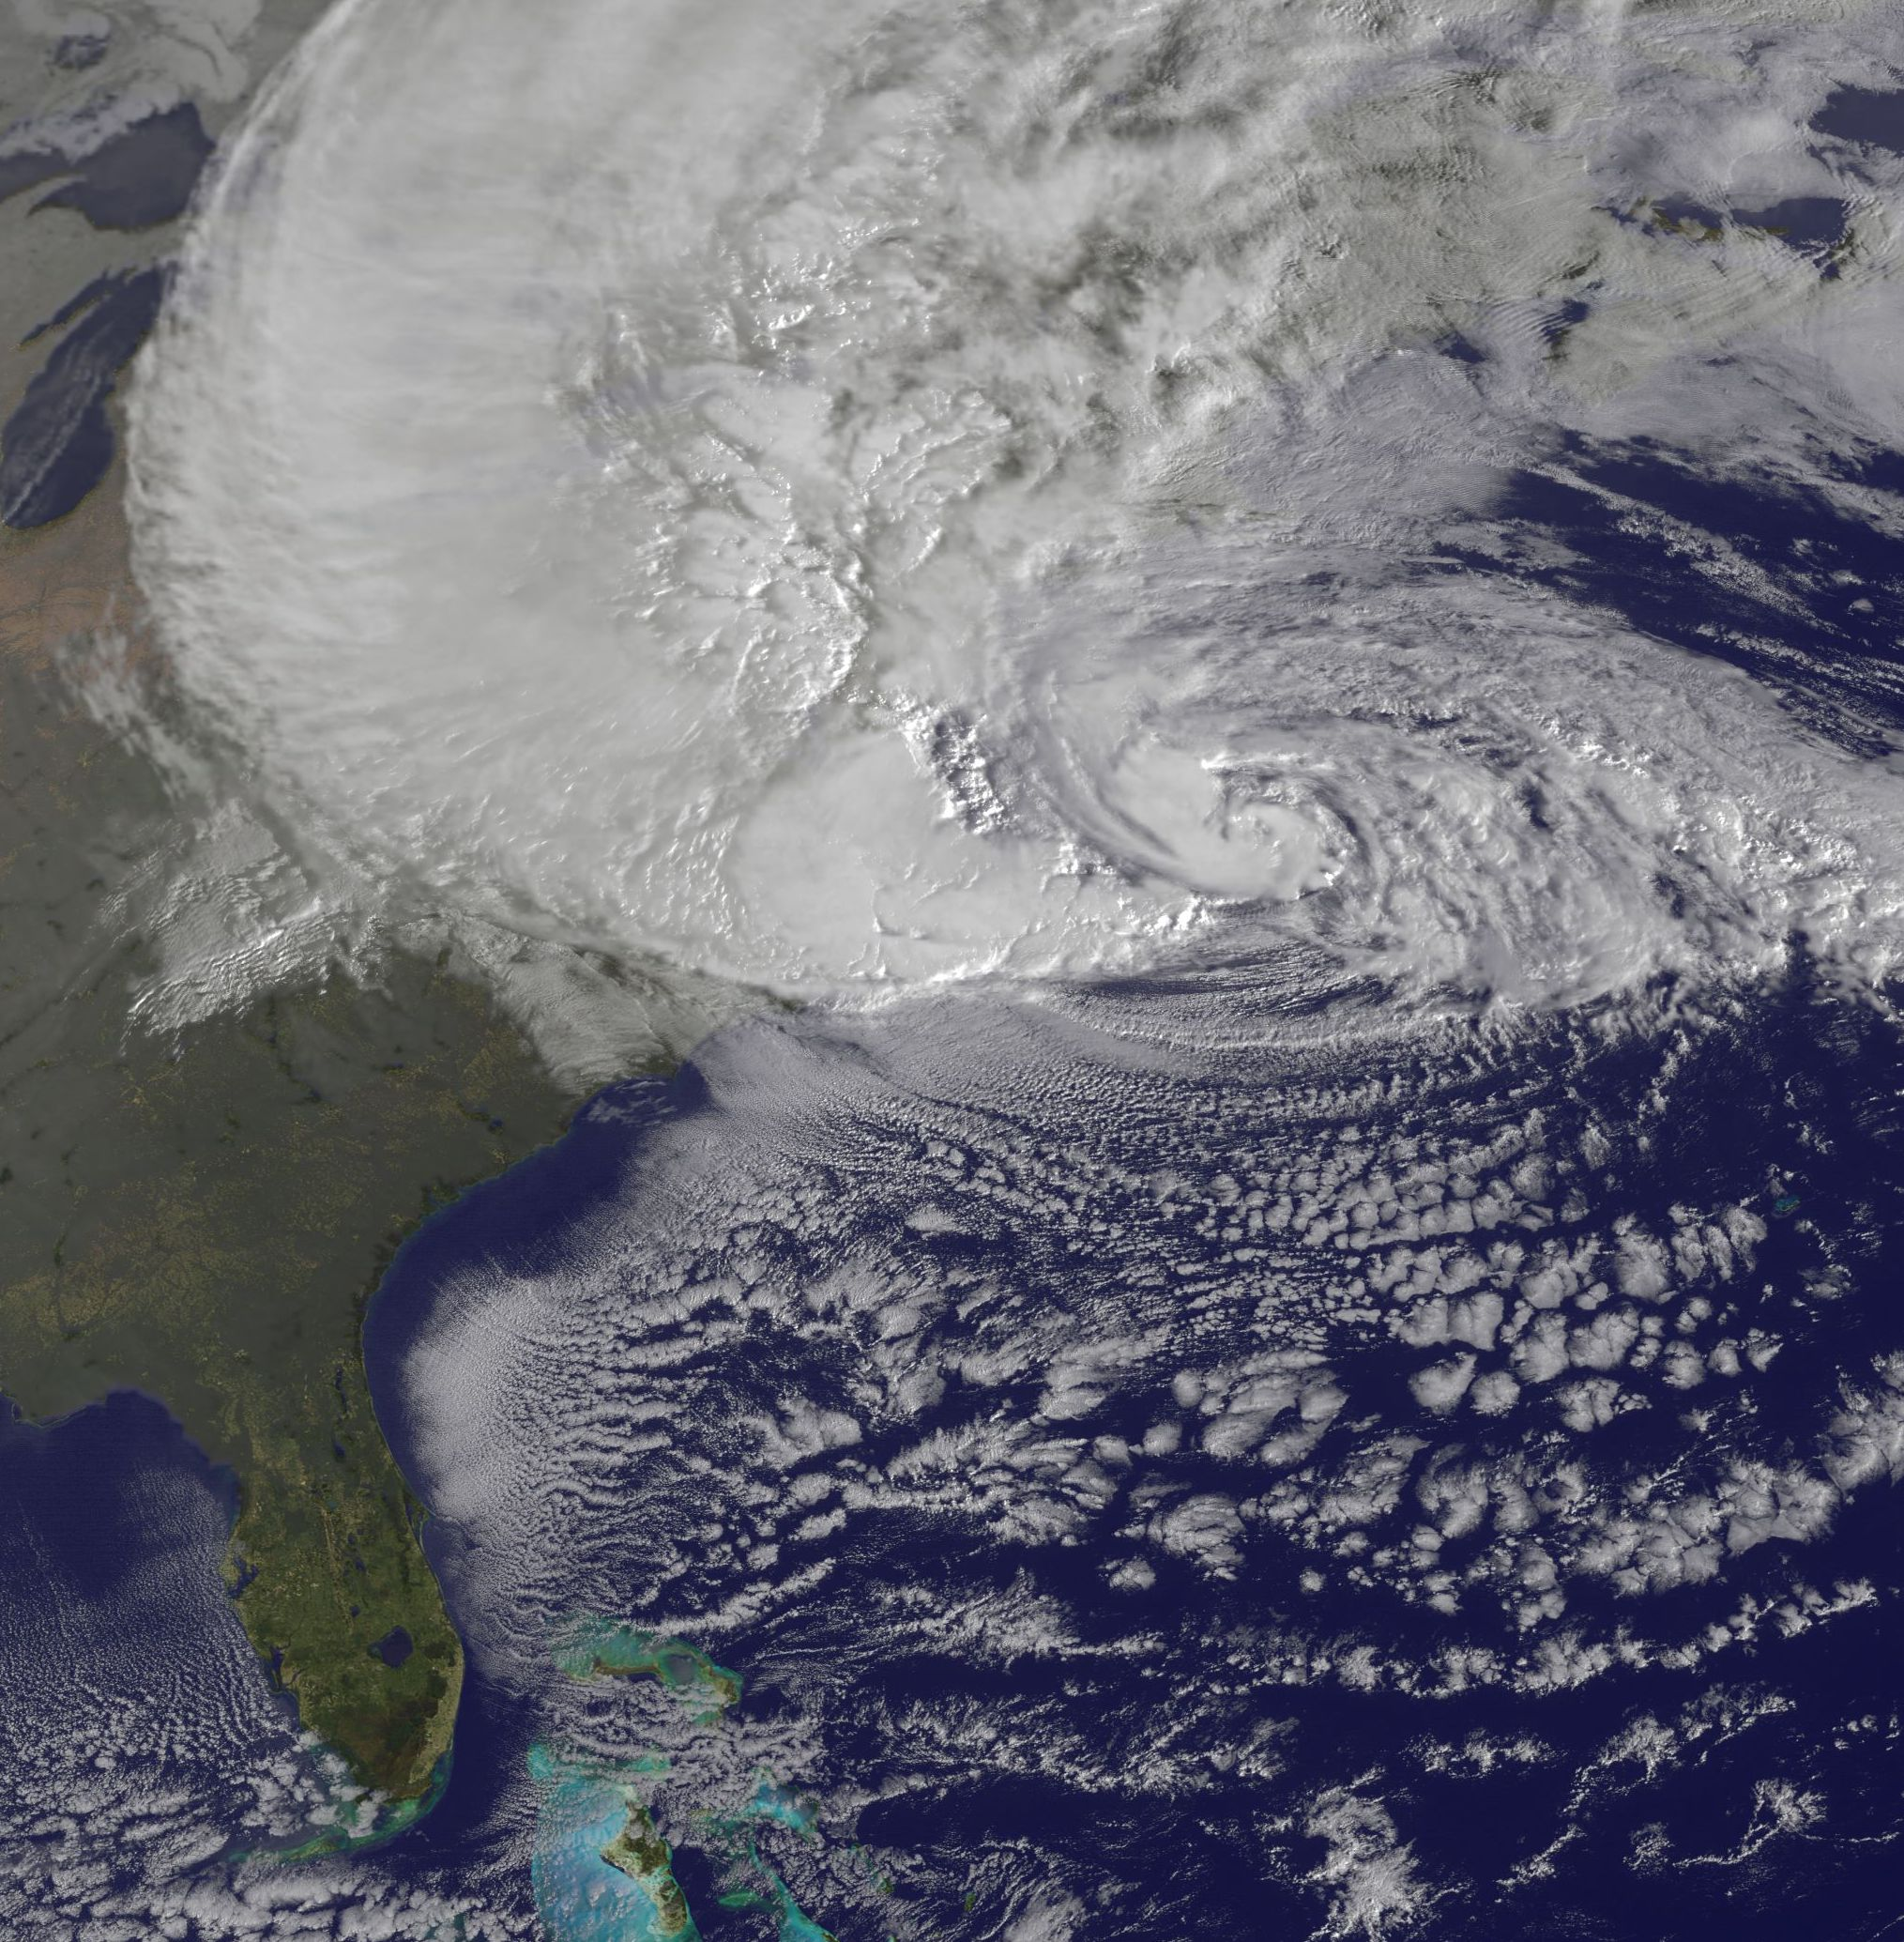
\includegraphics[width=\textwidth]{sandy_satellite} \end{center}
\vspace{-0.5cm}
\begin{center}
\scriptsize Source: NOAA / NASA GOES Project
\end{center}
\end{column}

\begin{column}{0.55\textwidth}
\small
\begin{block}{Health risks in storm-affected areas}
\begin{itemize}
  \item Change in patterns of emergency department visits (Kim et al. 2016)
  \item Increased outpatient cases of food and waterborne disease among elderly (Bloom et al. 2016)
  \item Increased rate of myocardial infarctions (Swerdel et al. 2014)
  \item Increased hospitalizations for dehydration (Lee et al. 2016)
  \item Difficulty obtaining medical care, medications, and medical equipment (Davidow et al. 2016)
\end{itemize}
\end{block}
\end{column}

\end{columns}

\end{frame}

\begin{frame}{Hazard-specific tropical storm metrics}

\begin{columns}
\begin{column}{0.5\textwidth}
\begin{block}{Tropical storm hazard metrics}
   \begin{itemize}
    \item Distance from the storm
    \item High winds
    \item Rainfall
    \item Storm surge
    \item Flood events
    \item Tornado events
   \end{itemize}
\end{block}
\end{column}
\begin{column}{0.5\textwidth}  
    \vspace{-0.25cm}
    \begin{center}
     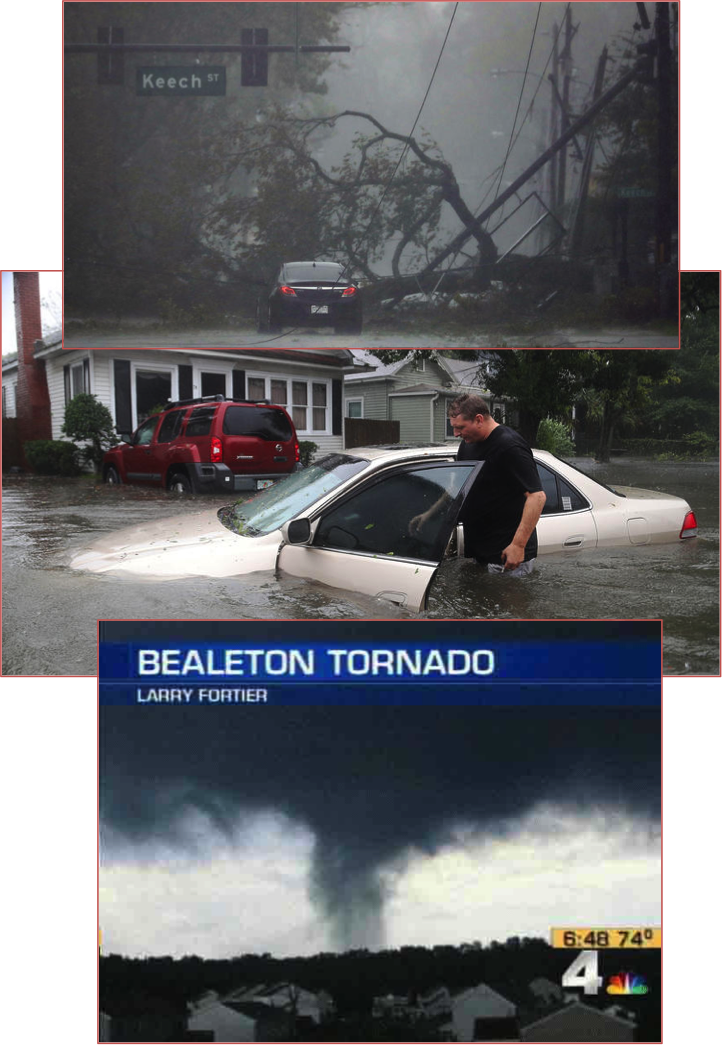
\includegraphics[width=0.8\textwidth]{storm_hazards.png}
     \end{center}
     \vspace{-0.25cm}
     \scriptsize{Image sources: Los Angeles Times, NBC}
\end{column}
\end{columns}

\end{frame}

\begin{frame}{Assessing tropical storm exposure}

\begin{block}{Challenge for epidemiological research}
How should we determine whether a county was exposed to a tropical storm for epidemiological research?
\end{block}

\vspace{-0.3cm}

\pause

\begin{center}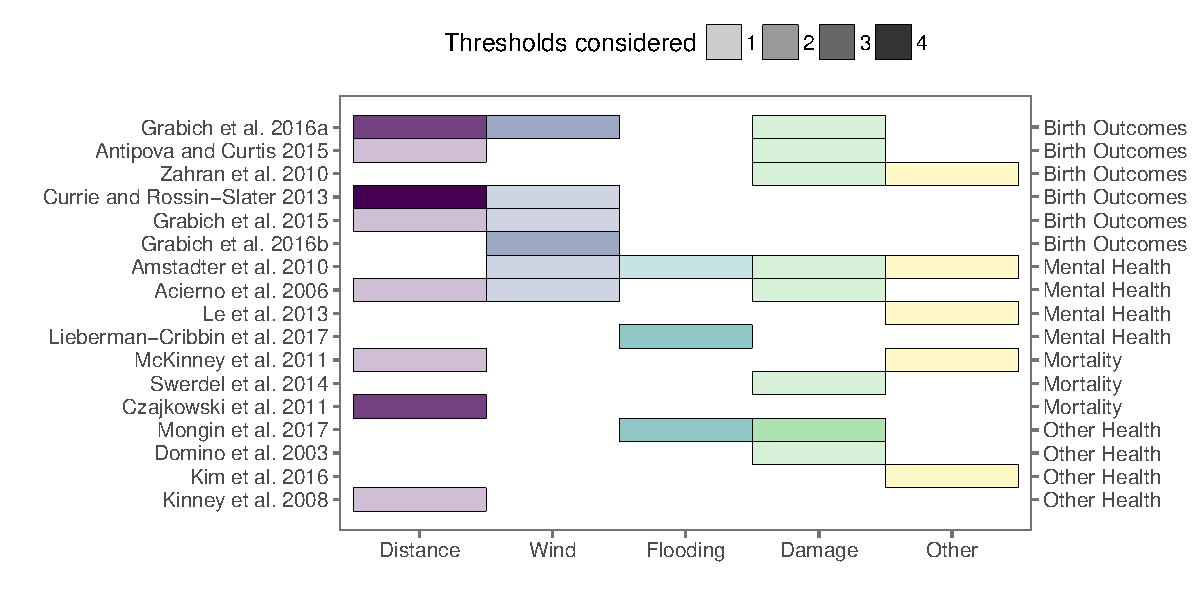
\includegraphics[height=0.77\textheight]{previous_exposure_metrics} \end{center}

\end{frame}

\begin{frame}{Project aims}

\begin{block}{Project aims}
\begin{itemize}
  \item Develop exposure classifications of all U.S. Atlantic basin tropical storms, 1996--2011, based on reasonable measurements of tropical storm hazards
  \item Assess agreement between hazard-based county-specific exposure classifications
  \item Make exposure assessments accessible to other researchers for epidemiological and other impact studies 
\end{itemize}
\end{block}

\end{frame}

\section{Assessing exposure}\label{assessing-exposure}

\begin{frame}{Assessing tropical storm exposure}

\begin{columns}
\begin{column}{0.5\textwidth}

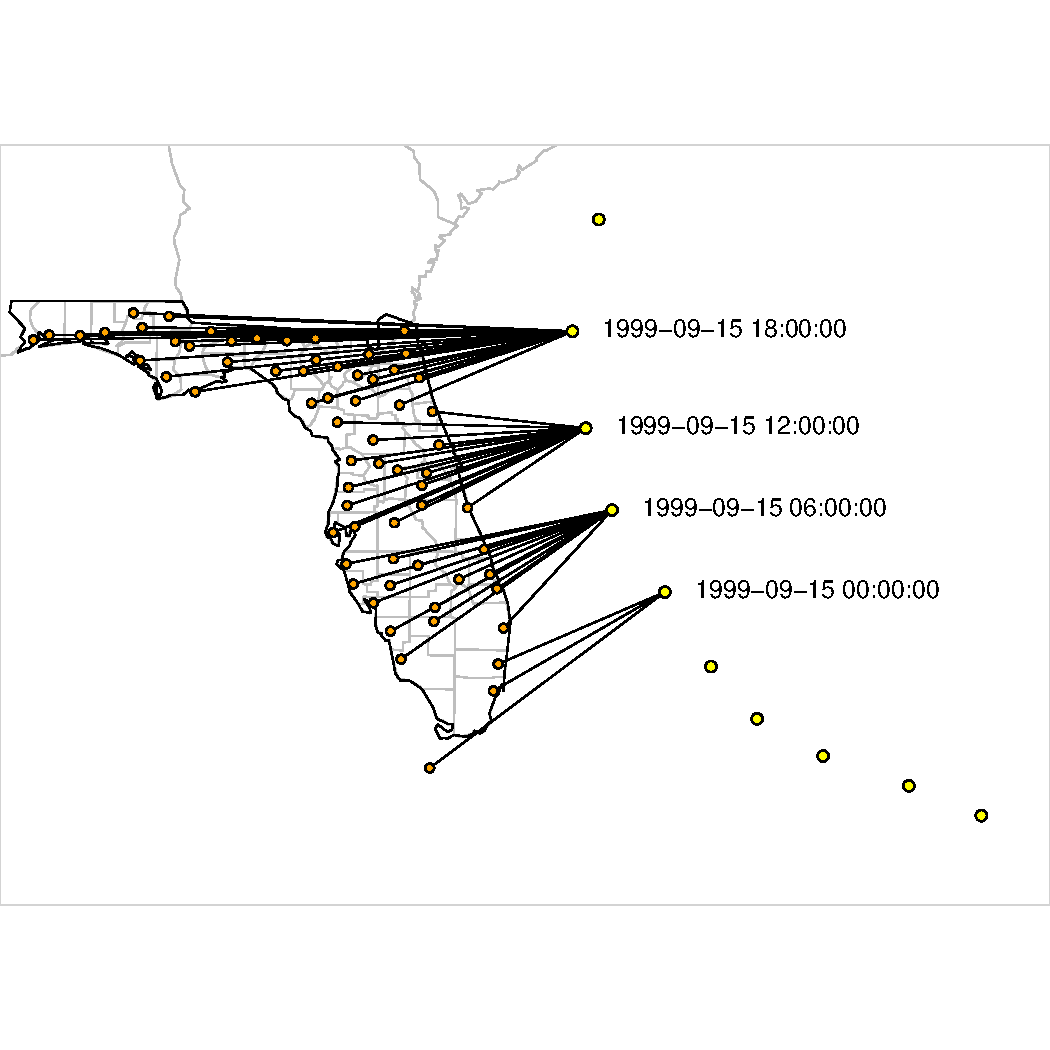
\includegraphics[width=\textwidth]{finding_closest_point} 

\vspace{-0.5cm}
\small
Example of "Best Tracks" data
\end{column}
\begin{column}{0.5\textwidth}
\small
\begin{block}{Distance metric}
\begin{itemize}
\item \textbf{Distance:} National Hurricane Center Best Tracks data
\item \textbf{Wind:} Wind model based on Willoughby et al. (2006)
\item \textbf{Rain:} Re-analysis rain data (NLDAS-2)
\item \textbf{Flood and tornado events:} NOAA Storm Events database
\end{itemize}
\end{block}
\end{column}
\end{columns}

\end{frame}

\begin{frame}{Rain exposure}

\begin{center}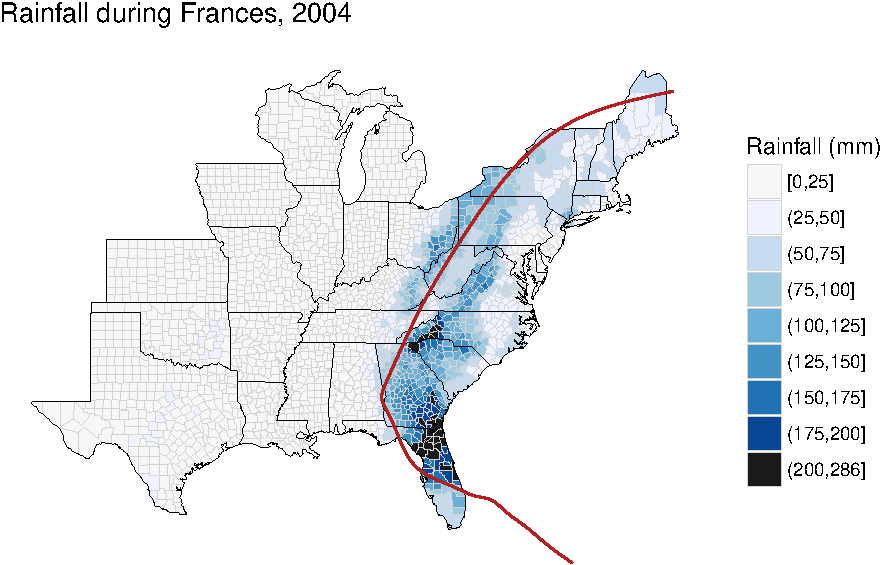
\includegraphics[width=0.9\textwidth]{anderson_apha_2017_files/figure-beamer/frances_rain_example-1} \end{center}

\end{frame}

\section{Agreement between exposure
metrics}\label{agreement-between-exposure-metrics}

\begin{frame}{County-level exposure to Hurricane Ivan (2004)}

\vspace{-0.6cm}

\begin{center}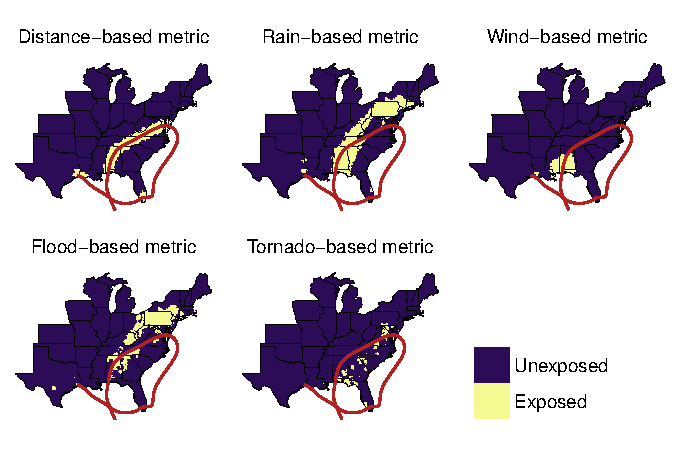
\includegraphics[height=0.75\textheight]{ivanexposurepresentation} \end{center}

\vspace{-0.5cm} \scriptsize Criteria for exposure classifications:
\textbf{Distance:} Within 100 kms of storm track. \textbf{Rain:} \(\ge\)
75 mm of rain total for two days before to one day after storm.
\textbf{Wind:} Modeled wind of \(\ge\) 15 m/s. \textbf{Flood, Tornado:}
Listed event in NOAA Storm Events database.

\end{frame}

\begin{frame}{County-level agreement in storm exposure}

\begin{block}{Assessing agreement in county classifications}
For each storm and each pair of metrics, we measured the \textit{Jaccard index} as a measure of county-level agreement in exposure classification for a storm:

\begin{equation*}
J = \frac{X_1 \cap X_2}{X_1 \cup X_2}
\end{equation*}

where $X_1$ is the set of counties exposed to a storm based on the first metric and $X_2$ is the set of counties exposed to the storm based on the second metric. 

\end{block}

\end{frame}

\begin{frame}{County-level agreement in storm exposure}

\vspace{-0.3cm}

\begin{center}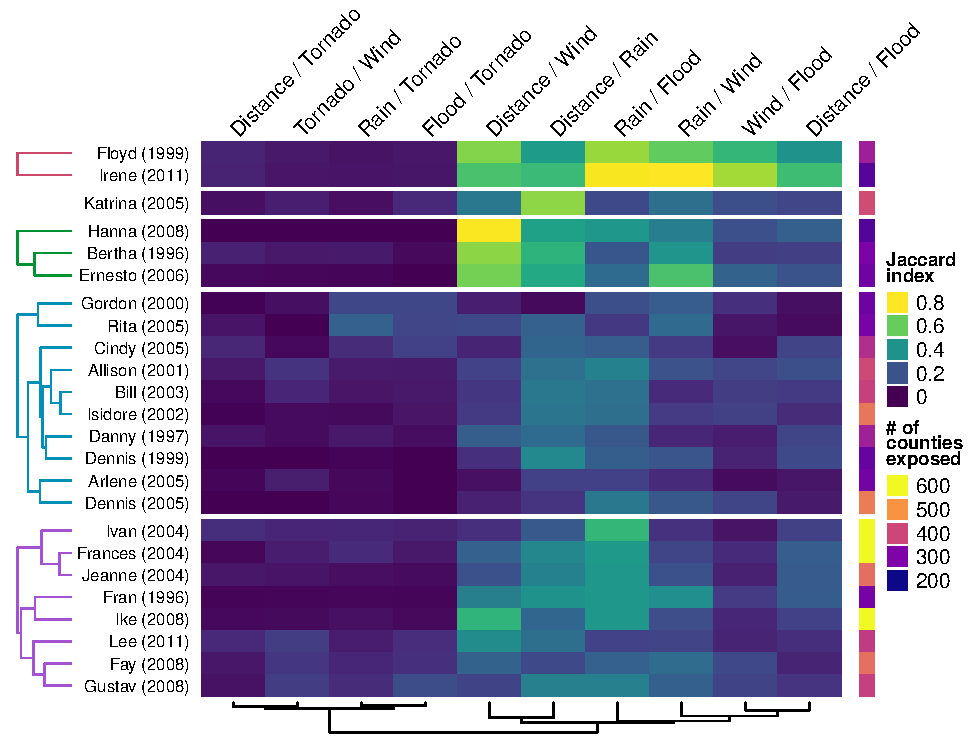
\includegraphics[height=0.87\textheight]{jaccard_heatmap_presentation} \end{center}

\end{frame}

\begin{frame}{Tropical storm exposure in U.S. counties}

\begin{centering}
\small Storm hits per county per decade based on rain (left) and wind (right) exposure metrics.
\end{centering}

\begin{center}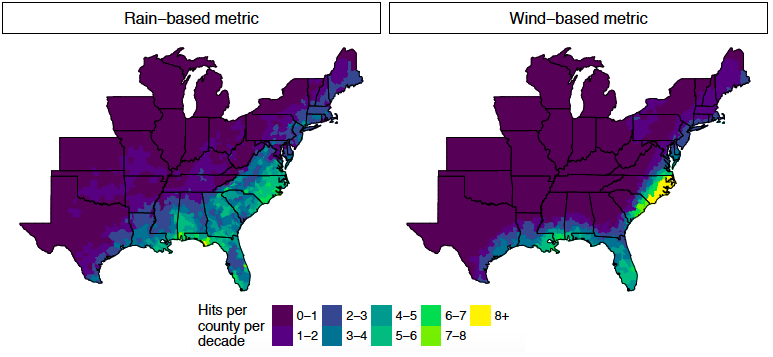
\includegraphics[width=0.95\textwidth]{hurricane_exposure} \end{center}

\vspace{-0.7cm} \scriptsize Criteria for exposure classifications:
\textbf{Rain:} \(\ge\) 75 mm of rain total for two days before to one
day after storm. \textbf{Wind:} Modeled wind of \(\ge\) 15 m/s.

\end{frame}

\section{Software}\label{software}

\begin{frame}[fragile]{Project software}

\footnotesize

\begin{block}{`hurricaneexposure`}
Create county-level exposure time series for tropical storms in U.S. counties. Exposure can be determined based on several hazards (e.g., distance, wind, rain), with user-specified thresholds. On CRAN.
\end{block}

\begin{Shaded}
\begin{Highlighting}[]
\KeywordTok{county_rain}\NormalTok{(}\DataTypeTok{counties =} \KeywordTok{c}\NormalTok{(}\StringTok{"22071"}\NormalTok{, }\StringTok{"51700"}\NormalTok{), }\DataTypeTok{rain_limit =} \DecValTok{100}\NormalTok{, }
            \DataTypeTok{start_year =} \DecValTok{1995}\NormalTok{, }\DataTypeTok{end_year =} \DecValTok{2005}\NormalTok{, }\DataTypeTok{dist_limit =} \DecValTok{100}\NormalTok{,}
            \DataTypeTok{days_included =} \KeywordTok{c}\NormalTok{(-}\DecValTok{1}\NormalTok{, }\DecValTok{0}\NormalTok{, }\DecValTok{1}\NormalTok{))}
\end{Highlighting}
\end{Shaded}

\begin{verbatim}
## # A tibble: 4 x 5
##       storm_id  fips closest_date storm_dist tot_precip
##          <chr> <chr>        <chr>      <dbl>      <dbl>
## 1    Bill-2003 22071   2003-06-30   38.78412      141.1
## 2 Charley-2004 51700   2004-08-14   43.01152      136.2
## 3   Cindy-2005 22071   2005-07-06   32.21758      113.2
## 4   Floyd-1999 51700   1999-09-16   46.50729      207.5
\end{verbatim}

\end{frame}

\begin{frame}{Project software}

\begin{columns}
\begin{column}{0.3\textwidth}
\footnotesize
\begin{block}{`stormwindmodel`}
Model storm winds from Best Tracks data at U.S. locations. Includes modeling sustained and gust winds, as well as duration of sustained and gust winds above a specified threshold. On CRAN.
\end{block}
\end{column}
\begin{column}{0.7\textwidth}

\begin{center}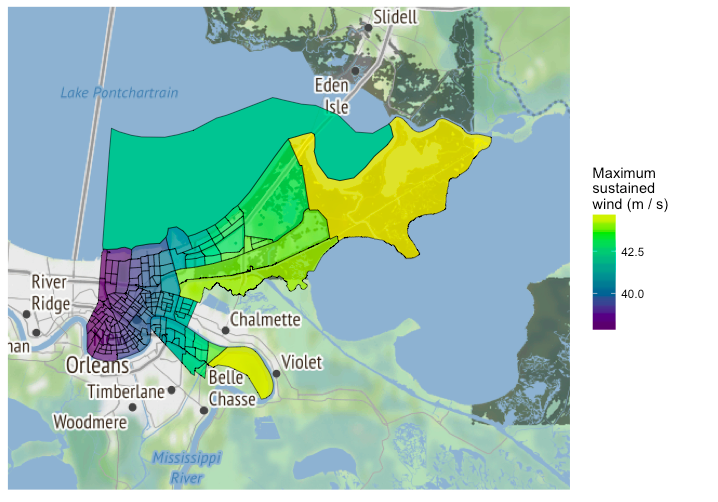
\includegraphics[width=\textwidth]{census_track_modeled_winds} \end{center}
\end{column}
\end{columns}

\end{frame}

\begin{frame}{Project software}

\footnotesize

\begin{block}{`countyweather`, `countyfloods`}
Download weather monitor data through NOAA and USGS APIs by U.S. county. Includes functions to map available monitors / gages for each county. On CRAN.
\end{block}

\footnotesize

\begin{block}{`noaastormevents`}
Download and explore listings from the NOAA Storm Events database. Includes the ability to pull events based on a tropical storm, using events listed close in time and distance to the storm's tracks. On CRAN.
\end{block}

\footnotesize

\begin{block}{`countytimezones`}
Convert time-stamps from UTC to local time zones for U.S. counties based on county FIPs. Facilitates merging weather observations with locally measured data, including health outcomes. On CRAN.
\end{block}

\end{frame}

\section{Conclusions}\label{conclusions}

\begin{frame}{Continuing work}

\begin{centering}
\small Relative risk for all-cause (left) and accidental (right) mortality in Miami, FL, at lags from the Hurricane Andrew storm day (lag 0) compared to non-storm days.
\end{centering}

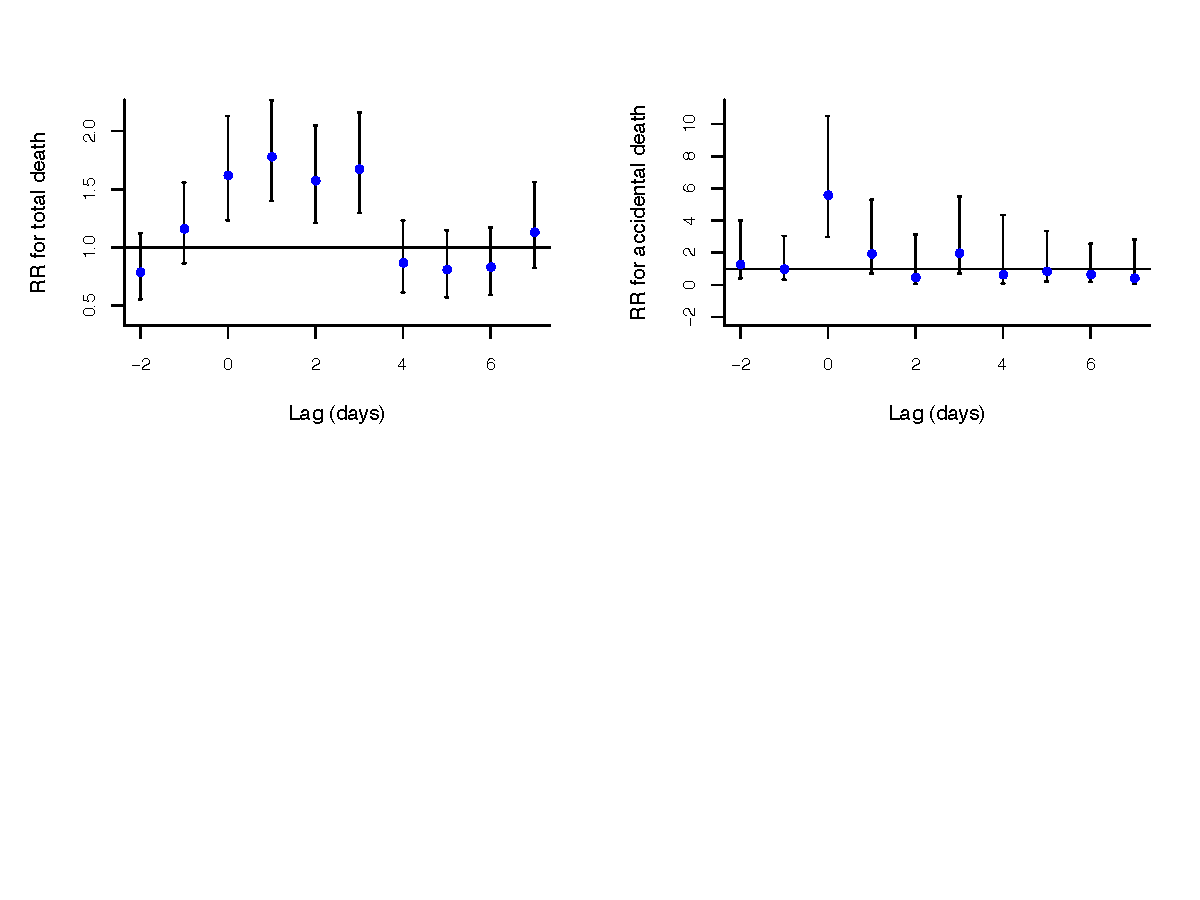
\includegraphics{miami_andrew_2.pdf}

\vspace{-0.2cm} \scriptsize Estimates were obtained by comparing storm
days to matched non-storm days in the same time of year and day of week
in other years. Matched days were picked to exclude days near other
storms. Lag 0 represents the storm day. Negative lags represent days
before the storm and positive lags represent days after the storm.
Vertical lines give 95\% confidence intervals.

\end{frame}

\begin{frame}{Acknowledgements}

\small

\begin{block}{Funding}
This work was supported in part by grants from the National Institute of Environmental Health Sciences (R00ES022631), the National Science Foundation (1331399), and a NASA Applied Sciences Program/Public Health Program Grant (NNX09AV81G).
\end{block}

\begin{block}{Collaborators}
Roger Peng, Meilin Yan, Joshua Ferreri, Dirk Eddelbuettel, Mohammad Al-Hamdan, William Crosson, Andrea Schumacher, Seth Guikema, and Steven Quiring collaborated on research and software shown here.
\end{block}

\end{frame}

\end{document}
